%% To submit your paper:
\documentclass[draft]{agujournal2019}
\usepackage{url} %this package should fix any errors with URLs in refs.
\usepackage{lineno}
\usepackage[inline]{trackchanges} %for better track changes. finalnew option will compile document with changes incorporated.
\usepackage{soul}
\linenumbers
%%%%%%%
% As of 2018 we recommend use of the TrackChanges package to mark revisions.
% The trackchanges package adds five new LaTeX commands:
%
%  \note[editor]{The note}
%  \annote[editor]{Text to annotate}{The note}
%  \add[editor]{Text to add}
%  \remove[editor]{Text to remove}
%  \change[editor]{Text to remove}{Text to add}
%
% complete documentation is here: http://trackchanges.sourceforge.net/
%%%%%%%

\draftfalse

\journalname{Geophysical Research Letters}


\begin{document}

%% ------------------------------------------------------------------------ %%
%  Title
%
% (A title should be specific, informative, and brief. Use
% abbreviations only if they are defined in the abstract. Titles that
% start with general keywords then specific terms are optimized in
% searches)
%
%% ------------------------------------------------------------------------ %%



\title{Duration of Individual Relativistic Electron Microbursts: A Probe Into Their Scattering Mechanism}

%% ------------------------------------------------------------------------ %%
%
%  AUTHORS AND AFFILIATIONS
%
%% ------------------------------------------------------------------------ %%

% Authors are individuals who have significantly contributed to the
% research and preparation of the article. Group authors are allowed, if
% each author in the group is separately identified in an appendix.)

% List authors by first name or initial followed by last name and
% separated by commas. Use \affil{} to number affiliations, and
% \thanks{} for author notes.
% Additional author notes should be indicated with \thanks{} (for
% example, for current addresses).

% Example: \authors{A. B. Author\affil{1}\thanks{Current address, Antartica}, B. C. Author\affil{2,3}, and D. E.
% Author\affil{3,4}\thanks{Also funded by Monsanto.}}

\authors{M. Shumko\affil{1}, L.W. Blum\affil{2}, and A.B. Crew\affil{3}}


\affiliation{1}{NASA's Goddard Space Flight Center, Greenbelt, Maryland}
\affiliation{2}{University of Colorado Boulder, Boulder, Colorado}
\affiliation{3}{Johns Hopkins University Applied Physics Laboratory, Laurel, Maryland}

\correspondingauthor{M. Shumko}{msshumko@gmail.com}

%% Keypoints, final entry on title page.

%  List up to three key points (at least one is required)
%  Key Points summarize the main points and conclusions of the article
%  Each must be 100 characters or less with no special characters or punctuation and must be complete sentences

\begin{keypoints}
\item We identified relativistic microbursts observed by the SAMPEX satellite and quantified their duration
\item Microburst duration roughly doubles between the midnight and noon magnetic local time regions
\item Whistler-mode chorus rising tone element \textcolor{red}{duration} has  a similar trend
\end{keypoints}

%% ------------------------------------------------------------------------ %%
%
%  ABSTRACT and PLAIN LANGUAGE SUMMARY
%
% A good Abstract will begin with a short description of the problem
% being addressed, briefly describe the new data or analyses, then
% briefly states the main conclusion(s) and how they are supported and
% uncertainties.

% The Plain Language Summary should be written for a broad audience,
% including journalists and the science-interested public, that will not have 
% a background in your field.
%
% A Plain Language Summary is required in GRL, JGR: Planets, JGR: Biogeosciences,
% JGR: Oceans, G-Cubed, Reviews of Geophysics, and JAMES.
% see http://sharingscience.agu.org/creating-plain-language-summary/)
%
%% ------------------------------------------------------------------------ %%

%% \begin{abstract} starts the second page

\begin{abstract}
In this study we used the Solar Anomalous and Magnetospheric Particle Explorer to identify relativistic, $>1$ MeV, microbursts and we quantified their duration. We found that the microburst duration is shortest near midnight magnetic local times and is longest, by a factor of two, near noon magnetic local times.
\end{abstract}

\section*{Plain Language Summary}
\noindent Microbursts are a naturally occurring form of electron precipitation from the near-Earth space into the atmosphere. They are characterized by their short duration, typically defined to be less than a second, or sometimes as 100 milliseconds... Microburst impact on the atmosphere includes the degradation of Mesospheric Ozone through the production of Odd Nitrogen and Odd Hydrogen molecules... We don't know the details on how microburst electrons are scattered, but there is evidence that they are scattered by whistler-mode chorus rising tone elements... Talk about duration and how it is a probe into the scattering physics.

\section{Introduction}\label{intro}
\textcolor{blue}{
\textbf{Outline}
\begin{enumerate}
    \item Introduce particle accelerating/scattering mechanism... dual role of chorus waves.
    \item One manifestation of electron-chorus scattering are electron microbursts.
    \item Briefly describe microbursts and their properties.
    \item Mention the chorus-microburst link, but it is currently unknown the physics of how electrons get scattered. Two approaches are quasi-linear diffusion and non-linear scatterring.
    \item Talk about microburst-chorus rising tone element duration and how they are similar. Mention the prior microburst width studies.
    \item The microburst width has not been explored as a function of geomagnetic indices or location.
    \item The trends in microburst width (duration) can be a probe into the conditions necessary to scatter microburst electrons.
\end{enumerate}
}

\section{Instrumentation}\label{instrumentation}
\textcolor{blue}{
\textbf{Outline}
\begin{enumerate}
    \item Describe SAMPEX
    \item Describe HILT
    \item Describe the 20 ms data used in this study (State4, 20 ms, avoided spin times). Data duration.
\end{enumerate}
}
In this study we used data taken by the Solar Anomalous Magnetospheric Particle Explorer (SAMPEX) satellite 

\section{Methodology}\label{methodology}
\textcolor{blue}{
\textbf{Outline}
\begin{enumerate}
    \item The methodology consists of two main steps: identify microbursts and estimate their duration.
    \item We identified microbursts using the Burst parameter. Mention the bias and how we addressed it.
    \item Discuss biases to short width, low counts. Douma 2019 showed that the microburst fluxes are roughly uniform in MLT (could this comparison be invalid since Douma also used the burst parameter?)
    \item Ref Fig 1 microbursts.
    \item Estimate microburst width using two methods:
    \item The prominence width method (cite my other paper).
    \item Gaussian + trend fit. Trend is important to approximate the drifting electrons in the DLC. automating fits is difficult so we helped out: the initial parameter guesses were provided from the prominence method, and the quality of fit checked with the $r^2$ and adj $r^2$. Provide the definition of $r^2$ used here and state the goodness of fit threshold we used.  
    \item Ref Fig 1 microbursts + fits. Mention the benefit of the linear trend, and screening out of multiple, superposed microbursts, by r2.
\end{enumerate}
}

To estimate the microburst duration we first identified microbursts and then we fit them with a Gaussian function.

\subsection{Microburst Identification}\label{microburst_id}
We identified microbursts using the burst parameter defined by \citeA{O'Brien2003} and used in numerous other microburst studies with SAMPEX \cite<e.g.>{Douma2017}. Assuming Poisson probability for the observed electron counts, the burst parameter is the number of standard deviations of a foreground signal above the background. It is generally defined as
\begin{equation}
bp = \frac{N-A}{\sqrt{A+1}}
\end{equation} \textcolor{red}{Find a better variable than bp. This is not British Petroleum} where $N$ is the number of foreground electron counts (microburst or otherwise), and $A$ is the centered running average counts representing the background. The $1$ in the denominator prevents a division by 0 error. In \citeA{O'Brien2003}, and in the figures in this study, $N$ was summed over 0.1 seconds and is called $N_{100}$, while $A$ parameter was summed over 0.5 seconds and is called $A_{500}$. Henceforth we will use the subscript for $N$ and $A$ for the time window used for the respective variables.

The choice of $A$ determines the sensitivity of the burst parameter to microbursts of various durations (widths). This sensitivity is best illustrated with an example. Given a 1-second wide microburst, if we use $A_{500}$, the centered average background at the microburst time is scewed higher towards the microburst peak. The average is dominated heavily by the microburst counts. On the other hand, if we use $A_{1000}$, the background will not be elevated as much because more true background counts will be included in the average. Therefore, $bp$ will be relatively larger for $A_{1000}$ than $A_{500}$. This sensitivity manifests itself as a bias towards narrower microbursts that we will address later in this study. 

\begin{figure}
\noindent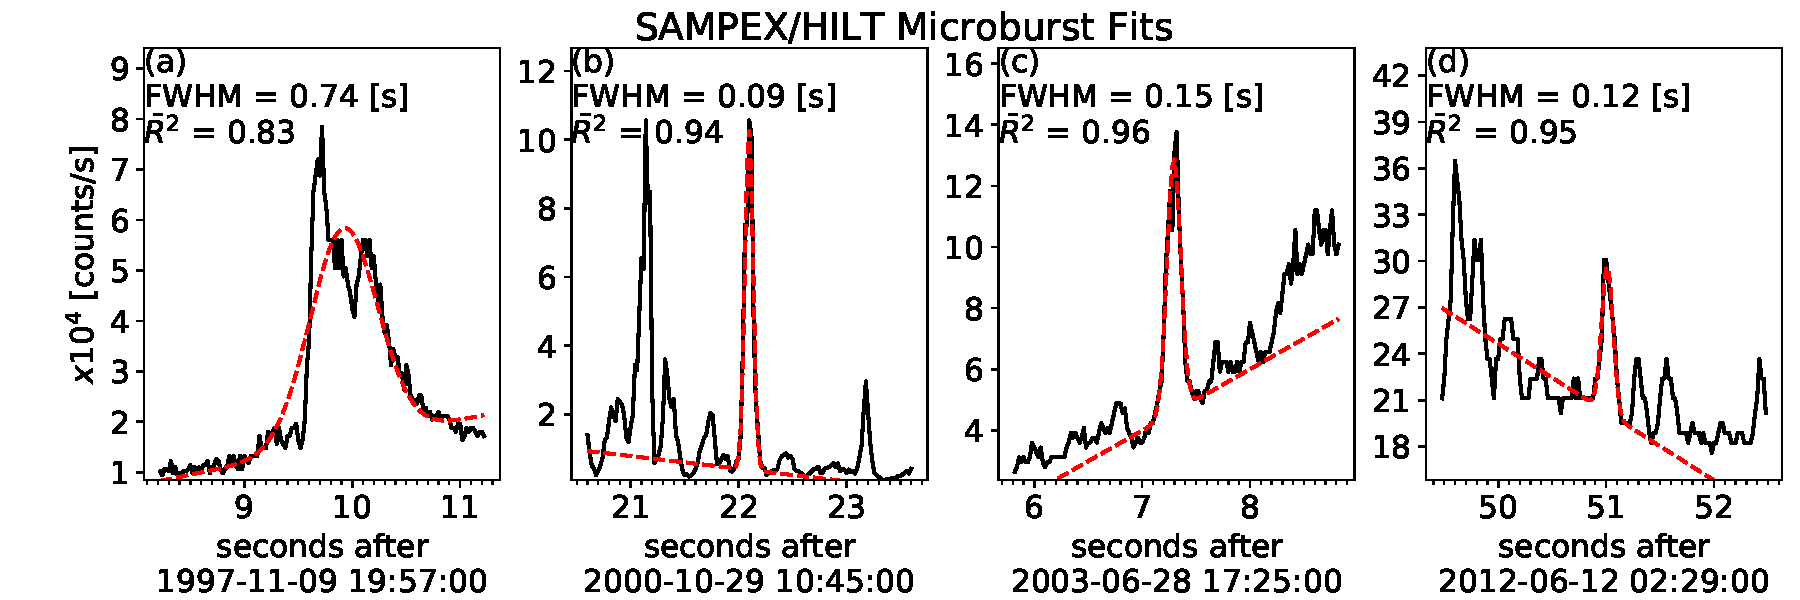
\includegraphics[width=\textwidth]{figures/fig1.pdf}
\caption{Example $>1$ MeV microbursts shown by the black lines, and the fits by the dashed red lines. The fit full width at half maximum (FWHM) and the $r^2$ goodness of fit score is annotated in each panel. In each panel, the major ticks are at every second, while the minor ticks are at every 100 milliseconds. Panel a shows how the $r^2$ score can screen out poor fits. The two superposed microbursts were fitted, but the $r^2$ score is less than the 0.9 threshold and so it was not analyzed in this study. Panels b, c and d show example of fits with $r^2$ values greater than 0.9 so therefore they were included in this analysis. Panels c and d demonstrate the necessity of the linear trend fit to account for the changing background.}
\label{fig1}
\end{figure}

\subsection{Microburst Duration}


\section{Results}\label{results}
\textcolor{blue}{
\textbf{Outline}
\begin{enumerate}
    \item Show the entire distrubution
    \item Show the L-MLT dial plots
    \item Show the marginalized distribution in MLT and L shell.
    \item Show the distribution with AE
\end{enumerate}
}

\begin{figure}
\noindent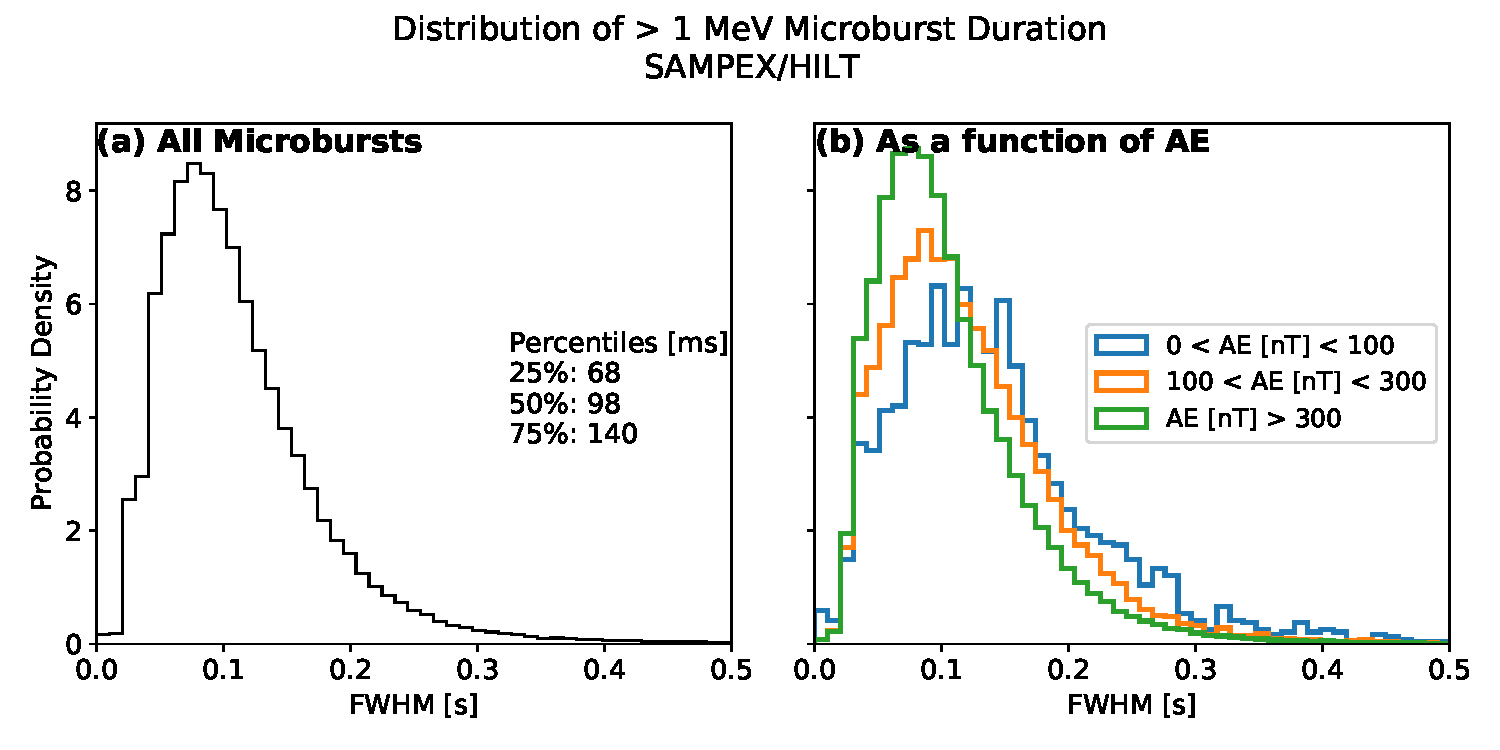
\includegraphics[width=\textwidth]{figures/fig2.pdf}
\caption{The joint distributions of microburst duration (FWHM) as a function of L and MLT. In each L-MLT bin with more than 100 good microburst fits, the 25th, 50th, and 75th percentiles of the duration were calculated and shown in panels a-c, respectively. The white bins in panels a-c have less than 100 good microburst fits. Panel d shows the distribution of the number of microbursts with 0 microbursts shown with the white bins.}
\label{fig2}
\end{figure}

\begin{figure}
\noindent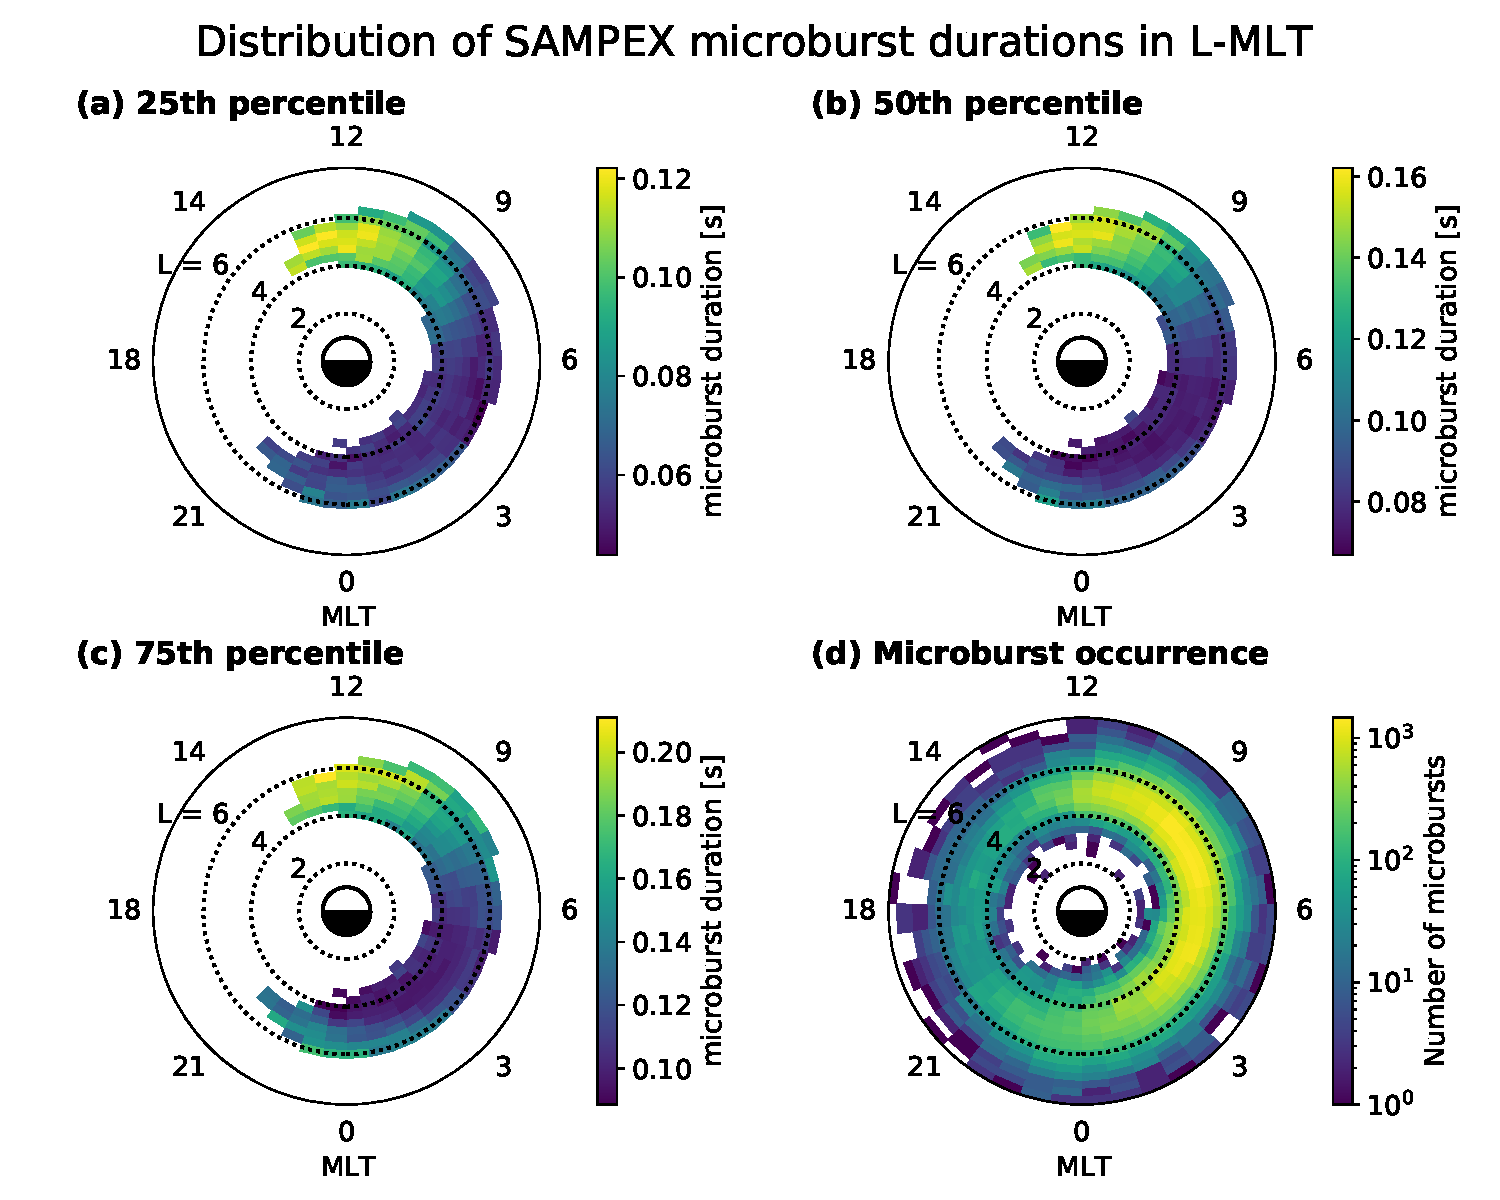
\includegraphics[width=\textwidth]{figures/fig3.pdf}
\caption{The marginalized distributions of the number of microbursts as a function of microburst duration (FWHM) and L shell in panel a and MLT in panel b.}
\label{fig3}
\end{figure}

\begin{figure}
\noindent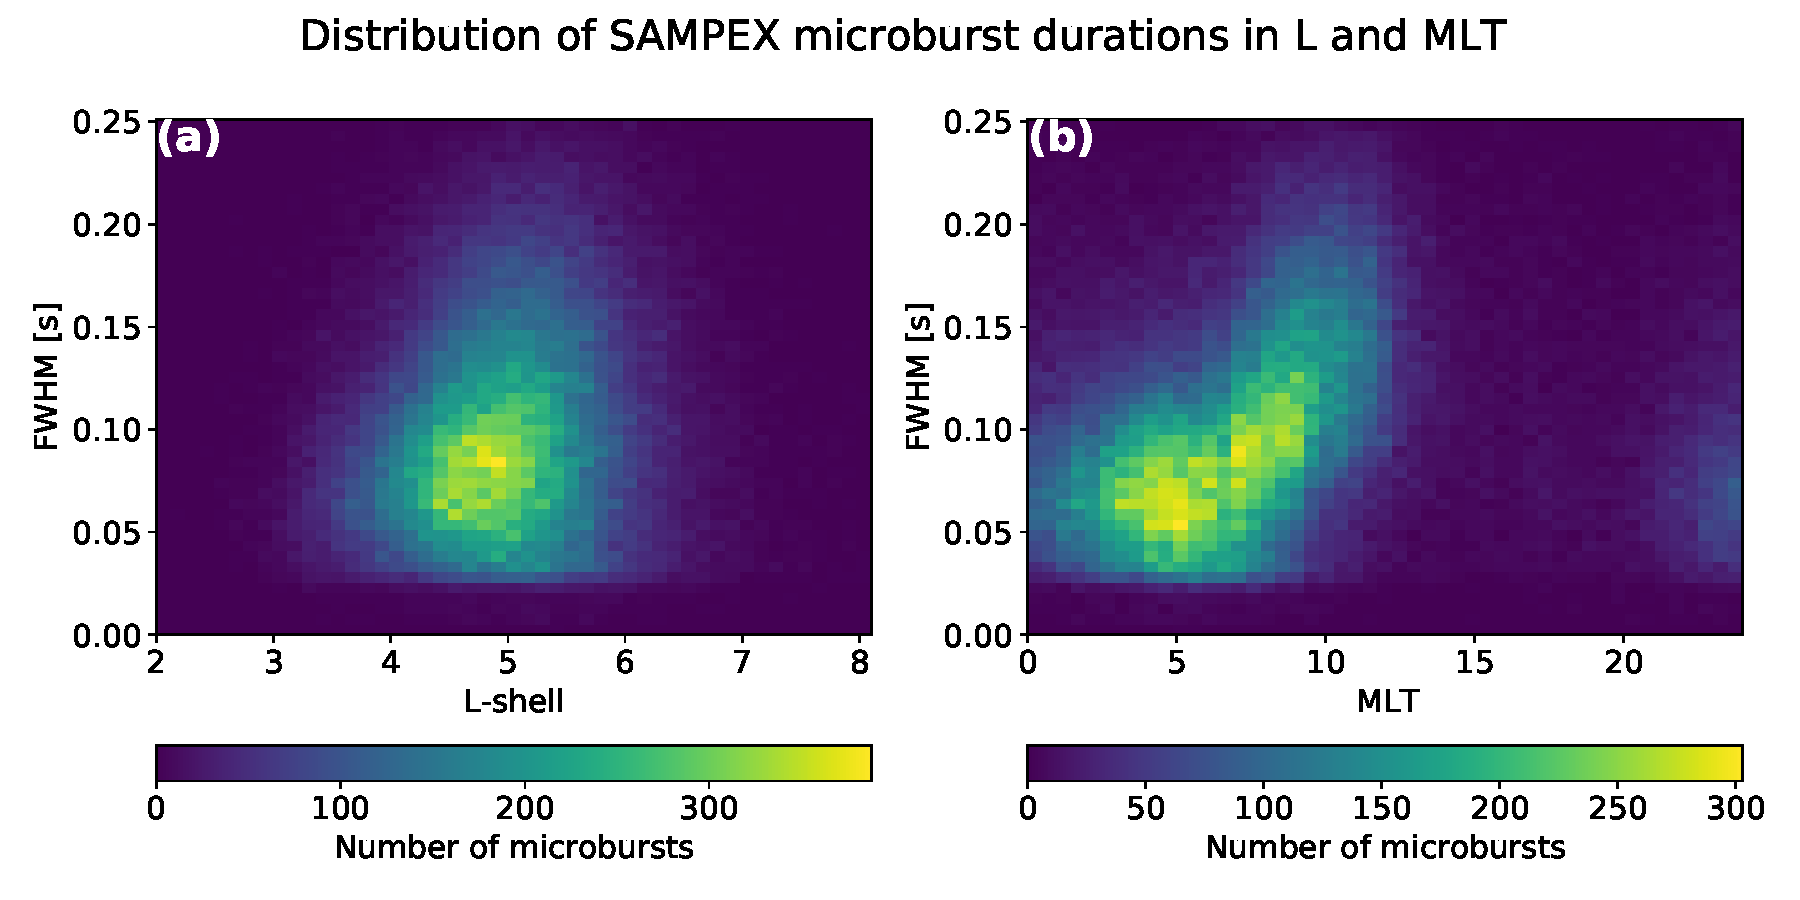
\includegraphics[width=\textwidth]{figures/fig4.pdf}
\caption{The distribution of the microburst duration (FWHM) for three ranges of the Auroral Electroject: $\mathrm{AE} < 100$, $100 < \mathrm{AE} < 300$, and $300 < \mathrm{AE} < 100$ nT in panels a-c, respectively. The y-axis probability density shares identical limits between the three panels.}
\label{fig3}
\end{figure}

\section{Discussion and Conclusions}\label{discussion}
\textcolor{blue}{
\textbf{Outline}
\begin{enumerate}
    \item Compare to prior microburst width estimates.
    \item Comment that microbursts at lower energy are wider (data + model). The cited microburst widths are dependent by the energy channel of the instrument. 
    \item Compare to chorus rising tone element duration trends.
    \item A few concluding remarks.
\end{enumerate}
}

To address the burst parameter preferential bias to narrower microbursts, as introduced in section \ref{microburst_id}, we ran the microburst identification algorithm on the data using three background values: $A_{500}$, $A_{1000}$, and $A_{1000}$. As described in section \ref{microburst_id}, an detection algorithm who's centered running average is over wider time periods will be more sensitive to wider and less prominent microbursts. Therefore we can identify the bias if there is a relative excess of longer duration microbursts when the average time was increased. We found no such excess for microburst data sets that were made using $A_{1000}$, and $A_{1000}$. Therefore, we believe that $>1$ MeV microbursts are truly narrower than 250 ms and the $A_{500}$ is adequate to identify $>1$ MeV microbursts.

%%%%%%%%%%%%%%%%%%%%%%%%%%%%%%%%
%% Optional Appendix goes here
%
% The \appendix command resets counters and redefines section heads
%
% After typing \appendix
%
%\section{Here Is Appendix Title}
% will show
% A: Here Is Appendix Title
%
%\appendix
%\section{Here is a sample appendix}

\acknowledgments
We are thankful for the engineers and scientists who made the SAMPEX mission possible. M. Shumko is thankful for the support provided by the NASA Postdoctoral Program at the NASA’s Goddard Space Flight Center, administered by Universities Space Research Association under contract with NASA. \textcolor{red}{Lauren's and Alex's funding sources} The SAMPEX HILT and attitude data are located at \url{http://www.srl.caltech.edu/sampex/DataCenter/data.html} and the minute cadence Auroral Electroject data is located at \url{ftp://ftp.ngdc.noaa.gov/STP/GEOMAGNETIC_DATA/INDICES/AURORAL_ELECTROJET/ONE_MINUTE/}.
The analysis software is archived at \textcolor{red}{\url{https://github.com/mshumko/sampex_microburst_widths}}.


%% ------------------------------------------------------------------------ %%
%% References and Citations

%%%%%%%%%%%%%%%%%%%%%%%%%%%%%%%%%%%%%%%%%%%%%%%
%
% \bibliography{<name of your .bib file>} don't specify the file extension
%
% don't specify bibliographystyle
%%%%%%%%%%%%%%%%%%%%%%%%%%%%%%%%%%%%%%%%%%%%%%%

\bibliography{refs.bib}



%Reference citation instructions and examples:
%
% Please use ONLY \cite and \citeA for reference citations.
% \cite for parenthetical references
% ...as shown in recent studies (Simpson et al., 2019)
% \citeA for in-text citations
% ...Simpson et al. (2019) have shown...
%
%
%...as shown by \citeA{jskilby}.
%...as shown by \citeA{lewin76}, \citeA{carson86}, \citeA{bartoldy02}, and \citeA{rinaldi03}.
%...has been shown \cite{jskilbye}.
%...has been shown \cite{lewin76,carson86,bartoldy02,rinaldi03}.
%... \cite <i.e.>[]{lewin76,carson86,bartoldy02,rinaldi03}.
%...has been shown by \cite <e.g.,>[and others]{lewin76}.
%
% apacite uses < > for prenotes and [ ] for postnotes
% DO NOT use other cite commands (e.g., \citet, \citep, \citeyear, \nocite, \citealp, etc.).
%



\end{document}



More Information and Advice:

%% ------------------------------------------------------------------------ %%
%
%  SECTION HEADS
%
%% ------------------------------------------------------------------------ %%

% Capitalize the first letter of each word (except for
% prepositions, conjunctions, and articles that are
% three or fewer letters).

% AGU follows standard outline style; therefore, there cannot be a section 1 without
% a section 2, or a section 2.3.1 without a section 2.3.2.
% Please make sure your section numbers are balanced.
% ---------------
% Level 1 head
%
% Use the \section{} command to identify level 1 heads;
% type the appropriate head wording between the curly
% brackets, as shown below.
%
%An example:
%\section{Level 1 Head: Introduction}
%
% ---------------
% Level 2 head
%
% Use the \subsection{} command to identify level 2 heads.
%An example:
%\subsection{Level 2 Head}
%
% ---------------
% Level 3 head
%
% Use the \subsubsection{} command to identify level 3 heads
%An example:
%\subsubsection{Level 3 Head}
%
%---------------
% Level 4 head
%
% Use the \subsubsubsection{} command to identify level 3 heads
% An example:
%\subsubsubsection{Level 4 Head} An example.
%
%% ------------------------------------------------------------------------ %%
%
%  IN-TEXT LISTS
%
%% ------------------------------------------------------------------------ %%
%
% Do not use bulleted lists; enumerated lists are okay.
% \begin{enumerate}
% \item
% \item
% \item
% \end{enumerate}
%
%% ------------------------------------------------------------------------ %%
%
%  EQUATIONS
%
%% ------------------------------------------------------------------------ %%

% Single-line equations are centered.
% Equation arrays will appear left-aligned.

Math coded inside display math mode \[ ...\]
 will not be numbered, e.g.,:
 \[ x^2=y^2 + z^2\]

 Math coded inside \begin{equation} and \end{equation} will
 be automatically numbered, e.g.,:
 \begin{equation}
 x^2=y^2 + z^2
 \end{equation}


% To create multiline equations, use the
% \begin{eqnarray} and \end{eqnarray} environment
% as demonstrated below.
\begin{eqnarray}
  x_{1} & = & (x - x_{0}) \cos \Theta \nonumber \\
        && + (y - y_{0}) \sin \Theta  \nonumber \\
  y_{1} & = & -(x - x_{0}) \sin \Theta \nonumber \\
        && + (y - y_{0}) \cos \Theta.
\end{eqnarray}

%If you don't want an equation number, use the star form:
%\begin{eqnarray*}...\end{eqnarray*}

% Break each line at a sign of operation
% (+, -, etc.) if possible, with the sign of operation
% on the new line.

% Indent second and subsequent lines to align with
% the first character following the equal sign on the
% first line.

% Use an \hspace{} command to insert horizontal space
% into your equation if necessary. Place an appropriate
% unit of measure between the curly braces, e.g.
% \hspace{1in}; you may have to experiment to achieve
% the correct amount of space.


%% ------------------------------------------------------------------------ %%
%
%  EQUATION NUMBERING: COUNTER
%
%% ------------------------------------------------------------------------ %%

% You may change equation numbering by resetting
% the equation counter or by explicitly numbering
% an equation.

% To explicitly number an equation, type \eqnum{}
% (with the desired number between the brackets)
% after the \begin{equation} or \begin{eqnarray}
% command.  The \eqnum{} command will affect only
% the equation it appears with; LaTeX will number
% any equations appearing later in the manuscript
% according to the equation counter.
%

% If you have a multiline equation that needs only
% one equation number, use a \nonumber command in
% front of the double backslashes (\\) as shown in
% the multiline equation above.

% If you are using line numbers, remember to surround
% equations with \begin{linenomath*}...\end{linenomath*}

%  To add line numbers to lines in equations:
%  \begin{linenomath*}
%  \begin{equation}
%  \end{equation}
%  \end{linenomath*}



